%\documentclass[hyperref={pdfpagelabels=false},slidetop,9pt]{beamer}
\documentclass[slidetop,8pt]{beamer}
\usepackage[T1]{fontenc}
\usepackage[utf8]{inputenc}
\newcommand{\id}{54}
\newcommand{\nom}{Liaisons mécaniques}
\newcommand{\sequence}{04}
\newcommand{\num}{01}
\newcommand{\type}{TP}
\newcommand{\descrip}{Modélisation d'un solide. Comportement des liaisons mécaniques. Modéliser les mécanismes du laboratoire par un schéma cinématique, paramétré.}
\newcommand{\competences}{A3-C4: Analyse d'architecture et de comportement \\ &  Mod1-C1: Isolement d'un solide ou d'un système de solides \\ &  Mod2-C10-1: Modèle de solide indéformable \\ &  Mod2-C11: Modélisation géométrique et cinématique des mouvements entre solides indéformables \\ &  Mod2-C12: Modélisation cinématique des liaisons entre solides \\ &  Mod2-C15: Modélisation des actions mécaniques \\ &  Rés-C6: Utilisation d'un solveur ou d'un logiciel multi physique \\ &  Com1-C1: Différents descripteurs introduits dans le programme \\ &  Com2-C4: Outils de communication}
\newcommand{\nbcomp}{9}
\newcommand{\systemes}{Plateforme Stewart}
\newcommand{\systemessansaccent}{Plateforme Stewart}
\newcommand{\ilot}{2}
\newcommand{\ilotstr}{02}
\newcommand{\dossierilot}{\detokenize{Ilot_02 Plateforme Stewart}}
\newcommand{\imageun}{Plateforme}

\newcommand{\urlsysteme}{\href{https://www.costadoat.fr/systeme/57}{Ressources système}}
\newcommand{\matlabsimscape}{\href{https://github.com/Costadoat/Sciences-Ingenieur/raw/master/Systemes/Plateforme Stewart/Plateforme_Stewart_Simscape.zip}{Modèle Simscape}}
\newcommand{\solidworks}{\href{https://github.com/Costadoat/Sciences-Ingenieur/raw/master/Systemes/Plateforme Stewart/Plateforme_Stewart_Solidworks.zip}{Modèle Solidworks}}
\newcommand{\edrawings}{\href{https://github.com/Costadoat/Sciences-Ingenieur/raw/master/Systemes/Plateforme Stewart/Plateforme_Stewart.EASM}{Modèle eDrawings}}
\newcommand{\test}{Stewart_param1}
\newcommand{\testi}{Stewart_param2}
\newcommand{\testii}{Stewart_param3}
\newcommand{\testiii}{Stewart_param4}
\newcommand{\testiiii}{Stewart_euler}
\usepackage{etex}
\usepackage{tikz}
\usepackage[european]{circuitikz}
\usepackage{pgf}
\usepackage[all]{xy}
\usepackage{pgfpages}
\usepackage{graphbox}
\usepackage{pdfpages}
\usepackage[adobe-utopia]{mathdesign}
\usepackage{ifthen}
\usepackage{cancel}
\usepackage{framed}
\usepackage{subfig}
\usepackage{tabularx}
\usepackage{setspace}
\usepackage{soul}
\usepackage{schemabloc}
\usepackage{eqnarray}
\usepackage[dot, phantomtext]{dashundergaps}
\usepackage{media9}
\usepackage{multimedia}
\usepackage{textcomp}

\author{Renaud Costadoat}
\institute{Lycée Dorian}

\usepackage{multido}
\usepackage{multirow}
\usepackage{multicol} % Portions de texte en colonnes
\usepackage{flafter}%floatants après la référence

\usepackage{color}
\usepackage{xcolor}
\usepackage{colortbl}

\usepackage[gen]{eurosym}
\usepackage{tikz}
%\usepackage{pstricks,pst-node,pst-tree,pst-solides3d}
\usepackage{lmodern}
\usepackage[francais]{babel}
\usepackage{pslatex}
\usetheme{renaud}
\usepackage{times}
\usepackage{amsmath}
\usepackage{verbatim}
\usepackage{moreverb}
%\usetikzlibrary{arrows,shapes}
\usepackage{graphicx}
\usepackage{psfrag}
\usepackage{wrapfig}
\usepackage{etoolbox}

\definecolor{gris25}{gray}{0.75}
\definecolor{bleu}{RGB}{18,33,98}
\definecolor{bleuf}{RGB}{42,94,171}
\definecolor{bleuc}{RGB}{231,239,247}
\definecolor{rougef}{RGB}{185,18,27}
\definecolor{rougec}{RGB}{255,188,204}%255,230,231
\definecolor{vertf}{RGB}{103,126,82}
\definecolor{vertc}{RGB}{220,255,191}

\setlength\parindent{24pt}
\parskip 7.2pt
\parindent 8pt

\newenvironment{rem}[1][\hsize]%
{%
    \def\FrameCommand
   {%
\rotatebox{90}{\textit{\textsf{Remarque}}} 
       {\color{bleuf}\vrule width 3pt}%
       \hspace{0pt}%must no space.
       \fboxsep=\FrameSep\colorbox{bleuc}%
  }%
    \MakeFramed{\hsize#1\advance\hsize-\width\FrameRestore}%
}%
{\endMakeFramed}%


\newenvironment{savoir}[1][\hsize]%
{%
    \def\FrameCommand
    {%
\rotatebox{90}{\textit{\textsf{Savoir}}} 
        {\color{bleuf}\vrule width 3pt}%
        \hspace{0pt}%must no space.
        \fboxsep=\FrameSep\colorbox{bleuc}%
    }%
    \MakeFramed{\hsize#1\advance\hsize-\width\FrameRestore}%
}%
{\endMakeFramed}%

\newenvironment{prob}[1][\hsize]%
{%
    \def\FrameCommand%
    {%
\rotatebox{90}{\textit{\textsf{Problematique}}} 
        {\color{rougef}\vrule width 3pt}%
        \hspace{0pt}%must no space.
        \fboxsep=\FrameSep\colorbox{rougec}%
    }%
    \MakeFramed{\hsize#1\advance\hsize-\width\FrameRestore}%
}%
{\endMakeFramed}%

\newenvironment{obj}[1][\hsize]%
{%
    \def\FrameCommand%
    {%
\rotatebox{90}{\textit{\textsf{Objectif}}} 
        {\color{vertf}\vrule width 3pt}%
        \hspace{0pt}%must no space.
        \fboxsep=\FrameSep\colorbox{vertc}%
    }%
    \MakeFramed{\hsize#1\advance\hsize-\width\FrameRestore}%
}%
{\endMakeFramed}%

\newenvironment{defi}[1][\hsize]%
{%
    \def\FrameCommand%
    {%
\rotatebox{90}{\textit{\textsf{Definition}}} 
        {\color{bleuf}\vrule width 3pt}%
        \hspace{0pt}%must no space.
        \fboxsep=\FrameSep\colorbox{rougec}%
    }%
    \MakeFramed{\hsize#1\advance\hsize-\width\FrameRestore}%
}%
{\endMakeFramed}%


\newenvironment{hypo}[1][\hsize]%
{%
    \def\FrameCommand%
    {%
\rotatebox{90}{\textit{\textsf{Hypothèse\\}}} 
        {\color{bleuf}\vrule width 3pt}%
        \hspace{0pt}%must no space.
        \fboxsep=\FrameSep\colorbox{bleuc}%
    }%
    \MakeFramed{\hsize#1\advance\hsize-\width\FrameRestore}%
}%
{\endMakeFramed}%


\newenvironment{prop}[1][\hsize]%
{%
    \def\FrameCommand%
    {%
\rotatebox{90}{\textit{\textsf{Propriété}}} 
        {\color{bleuf}\vrule width 3pt}%
        \hspace{0pt}%must no space.
        \fboxsep=\FrameSep\colorbox{bleuc}%
    }%
    \MakeFramed{\hsize#1\advance\hsize-\width\FrameRestore}%
}%
{\endMakeFramed}%

\newenvironment{props}[1][\hsize]%
{%
    \def\FrameCommand%
    {%
\rotatebox{90}{\textit{\textsf{Propriétés}}} 
        {\color{bleuf}\vrule width 3pt}%
        \hspace{0pt}%must no space.
        \fboxsep=\FrameSep\colorbox{bleuc}%
    }%
    \MakeFramed{\hsize#1\advance\hsize-\width\FrameRestore}%
}%
{\endMakeFramed}%

\newenvironment{exemple}[1][\hsize]%
{%
    \def\FrameCommand%
    {%
\rotatebox{90}{\textit{\textsf{Exemple}}} 
        {\color{vertf}\vrule width 3pt}%
        \hspace{0pt}%must no space.
        \fboxsep=\FrameSep\colorbox{vertc}%
    }%
    \MakeFramed{\hsize#1\advance\hsize-\width\FrameRestore}%
}%
{\endMakeFramed}%

\newenvironment{resultat}[1][\hsize]%
{%
    \def\FrameCommand%
    {%
\rotatebox{90}{\textit{\textsf{Résultat}}} 
        {\color{rougef}\vrule width 3pt}%
%        {\color{bleuf}\vrule width 3pt}%
        \hspace{0pt}%must no space.
        \fboxsep=\FrameSep\colorbox{rougec}%
    }%
    \MakeFramed{\hsize#1\advance\hsize-\width\FrameRestore}%
}%
{\endMakeFramed}%

\newenvironment{methode}[1][\hsize]%
{%
    \def\FrameCommand%
    {%
\rotatebox{90}{\textit{\textsf{Méthode\\}}} 
        {\color{rougef}\vrule width 3pt}%
        \hspace{0pt}%must no space.
        \fboxsep=\FrameSep\colorbox{rougec}%
    }%
    \MakeFramed{\hsize#1\advance\hsize-\width\FrameRestore}%
}%
{\endMakeFramed}%

\newenvironment{theo}[1][\hsize]%
{%
    \def\FrameCommand%
    {%
\rotatebox{90}{\textit{\textsf{Théorème\\}}} 
        {\color{rougef}\vrule width 3pt}%
        \hspace{0pt}%must no space.
        \fboxsep=\FrameSep\colorbox{rougec}%
    }%
    \MakeFramed{\hsize#1\advance\hsize-\width\FrameRestore}%
}%
{\endMakeFramed}%

\newenvironment{warn}[1][\hsize]%
{%
    \def\FrameCommand%
    {%
\rotatebox{90}{\textit{\textsf{Attention\\}}} 
        {\color{rougef}\vrule width 3pt}%
        \hspace{0pt}%must no space.
        \fboxsep=\FrameSep\colorbox{rougec}%
    }%
    \MakeFramed{\hsize#1\advance\hsize-\width\FrameRestore}%
}%
{\endMakeFramed}%

% \usepackage{pstricks}
%\usepackage{minitoc}
% \setcounter{minitocdepth}{4}

\setcounter{tocdepth}{2}

% \mtcselectlanguage{french} 

%\usepackage{draftcopy}% "Brouillon"
% \usepackage{floatflt}
\usepackage{psfrag}
%\usepackage{listings} % Permet d'insérer du code de programmation
\renewcommand{\baselinestretch}{1.2}

% Changer la num�rotation des figures :
% ------------------------------------
% \makeatletter
% \renewcommand{\thefigure}{\ifnum \c@section>\z@ \thesection.\fi
%  \@arabic\c@figure}
% \@addtoreset{figure}{section}
% \makeatother
 


%%%%%%%%%%%%
% Définition des vecteurs %
%%%%%%%%%%%%
 \newcommand{\vect}[1]{\overrightarrow{#1}}

%%%%%%%%%%%%
% Définition des torseusr %
%%%%%%%%%%%%

 \newcommand{\torseur}[1]{%
\left\{{#1}\right\}
}

\newcommand{\torseurcin}[3]{%
\left\{\mathcal{#1} \left(#2/#3 \right) \right\}
}

\newcommand{\torseurstat}[3]{%
\left\{\mathcal{#1} \left(#2\rightarrow #3 \right) \right\}
}

 \newcommand{\torseurc}[8]{%
%\left\{#1 \right\}=
\left\{
{#1}
\right\}
 = 
\left\{%
\begin{array}{cc}%
{#2} & {#5}\\%
{#3} & {#6}\\%
{#4} & {#7}\\%
\end{array}%
\right\}_{#8}%
}

 \newcommand{\torseurcol}[7]{
\left\{%
\begin{array}{cc}%
{#1} & {#4}\\%
{#2} & {#5}\\%
{#3} & {#6}\\%
\end{array}%
\right\}_{#7}%
}

 \newcommand{\torseurl}[3]{%
%\left\{\mathcal{#1}\right\}_{#2}=%
\left\{%
\begin{array}{l}%
{#1} \\%
{#2} %
\end{array}%
\right\}_{#3}%
}

 \newcommand{\vectv}[3]{%
\vect{V\left( {#1} \in {#2}/{#3}\right)}
}


\newcommand{\vectf}[2]{%
\vect{R\left( {#1} \rightarrow {#2}\right)}
}

\newcommand{\vectm}[3]{%
\vect{\mathcal{M}\left( {#1}, {#2} \rightarrow {#3}\right)}
}


 \newcommand{\vectg}[3]{%
\vect{\Gamma \left( {#1} \in {#2}/{#3}\right)}
}

 \newcommand{\vecto}[2]{%
\vect{\Omega\left( {#1}/{#2}\right)}
}

\newcommand{\reponse}[1][4]
{
\multido{}{#1}
{
\begin{center}
\makebox[0.9\linewidth]{\dotfill} \end{center}
}}


% }$$\left\{\mathcal{#1} \right\}_{#2} =%
% \left\{%
% \begin{array}{c}%
%  #3 \\%
%  #4 %
% \end{array}%
% \right\}_{#5}}


%  ------------------------------------------
% | Modification du formatage des sections : | 
%  ------------------------------------------

% Grands titres :
% ---------------

\newcommand{\titre}[1]{%
\begin{center}
      \bigskip
      \rule{\textwidth}{1pt}
      \par\vspace{0.1cm}
      
      \textbf{\large #1}
      \par\rule{\textwidth}{1pt}
    \end{center}
    \bigskip
  }

% Supprime le numéro du chapitre dans la numérotation des sections:
% -----------------------------------------------------------------
\makeatletter
\renewcommand{\thesection}{\@arabic\c@section}
\makeatother


% \titleformat{\chapter}[display]
% {\normalfont\Large\filcenter}
% {}
% {1pc}
% {\titlerule[1pt]
%   \vspace{1pc}%
%   \Huge}[\vspace{1ex}%
% \titlerule]


%%%% Chapitres Comme PY Pechard %%%%%%%%%
% numéro du chapitre
\DeclareFixedFont{\chapnumfont}{OT1}{phv}{b}{n}{80pt}
% pour le mot " Chapitre "
\DeclareFixedFont{\chapchapfont}{OT1}{phv}{m}{it}{40pt}
% pour le titre
\DeclareFixedFont{\chaptitfont}{T1}{phv}{b}{n}{25pt}

\definecolor{gris}{gray}{0.75}
\setbeamertemplate{section in toc}[sections numbered]

\newlength{\RoundedBoxWidth}
\newsavebox{\GrayRoundedBox}
\newenvironment{GrayBox}[1][\dimexpr\textwidth-4.5ex]%
   {\setlength{\RoundedBoxWidth}{\dimexpr#1}
    \begin{lrbox}{\GrayRoundedBox}
       \begin{minipage}{\RoundedBoxWidth}}%
   {   \end{minipage}
    \end{lrbox}
    \begin{center}
    \begin{tikzpicture}%
       \draw node[draw=bleuf,fill=bleuc,rounded corners,%
             inner sep=2ex,text width=\RoundedBoxWidth]%
             {\usebox{\GrayRoundedBox}};
    \end{tikzpicture}
    \end{center}}
    
\ifdef{\prive}{\pgfpagesuselayout{2 on 1}[a4paper,border shrink=0mm]}
\ifdef{\prive}{\setbeamertemplate{navigation symbols}{}}
\setbeamertemplate{itemize item}[ball]
%\setbeamertemplate{blocks}[rounded]%[shadow=true]
\setbeamercolor{block title}{fg=white,bg=grisf}        % titre block normal 
\setbeamercolor{block body}{fg=grisf,bg=grisc!50}      % corps block normal
\setbeamercolor{block body alerted}{fg=white,bg=warning}   % idem pour un block alerte

\title{\nom}
\date{S\sequence \ - \type\num}

\begin{document}
\shorthandoff{:!}
\bibliographystyle{abbrvnat-fr}

\usebackgroundtemplate%
{%
    \centering
\includegraphics[width=\paperwidth]{../../img/fond2}%
}

{
\setbeamertemplate{navigation symbols}{}
\setbeamertemplate{headline}[pagetitre]
\setbeamertemplate{footline}[pagetitre]
\usebackgroundtemplate{\centering
\includegraphics[width=\paperwidth]{../../img/fond}}
\frame{\titlepage}
}



\setcounter{framenumber}{0}

{\frame{
\frametitle{Introduction}

\begin{savoir}
Vous êtes capables :
\begin{itemize}
 \item De définir le modèle nominal d'une pièce ou d'un assemblage,
 \item D'analyser un cahier des charges afin de déterminer les exigences sur une pièce.
\end{itemize}
\end{savoir}

\begin{prob}
Vous devez êtes capables :
\begin{itemize}
 \item De limiter les défauts acceptables d'une pièce,
 \item De spécifier une pièce sur un dessin.
\end{itemize}
\end{prob}
}}

\section{Introduction}

{\frame{
\frametitle{Écarts géométriques: le Jeu}

\textbf{Besoin} : Un mécanisme est conçu pour répondre à un besoin.

\begin{center}
 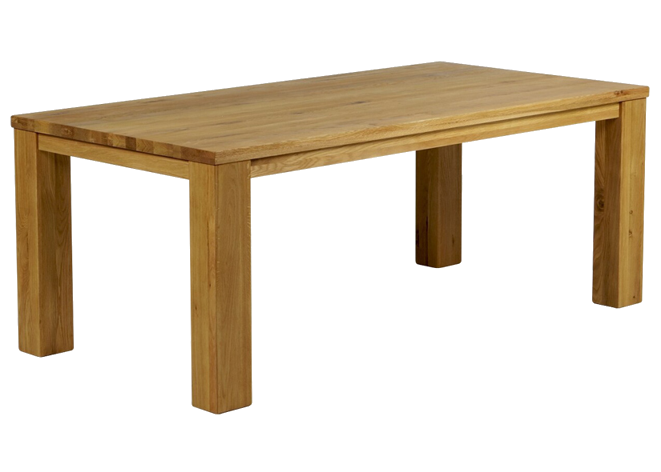
\includegraphics[width=0.5\linewidth]{img/Picture1}
\end{center}

\textit{Exemple} : Table basse. \\
\textit{Exigences} : 
\begin{itemize}
	\item Mettre un objet à hauteur d'homme,
	\item Positionner l'objet par rapport au sol.
\end{itemize}
}}

{\frame{
\frametitle{Conception}

\textbf{Conception} : Les composants du mécanismes sont utilisés pour répondre aux fonctions.

Pour positionner l'objet par rapport au sol, il faut le surélever par rapport au sol de 50 cm, il est nécessaire que les 4 pieds aient une longueur de 50 cm.

\textbf{Résultat de la conception:}\\
\begin{center}
 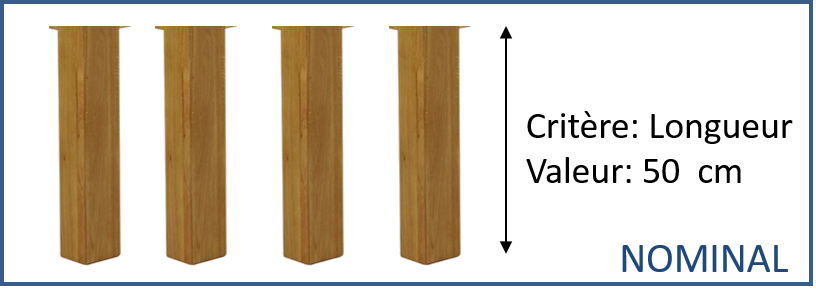
\includegraphics[width=0.5\linewidth]{img/Picture2}
\end{center}
}}

{\frame{
\frametitle{Fabrication}

\begin{center}
 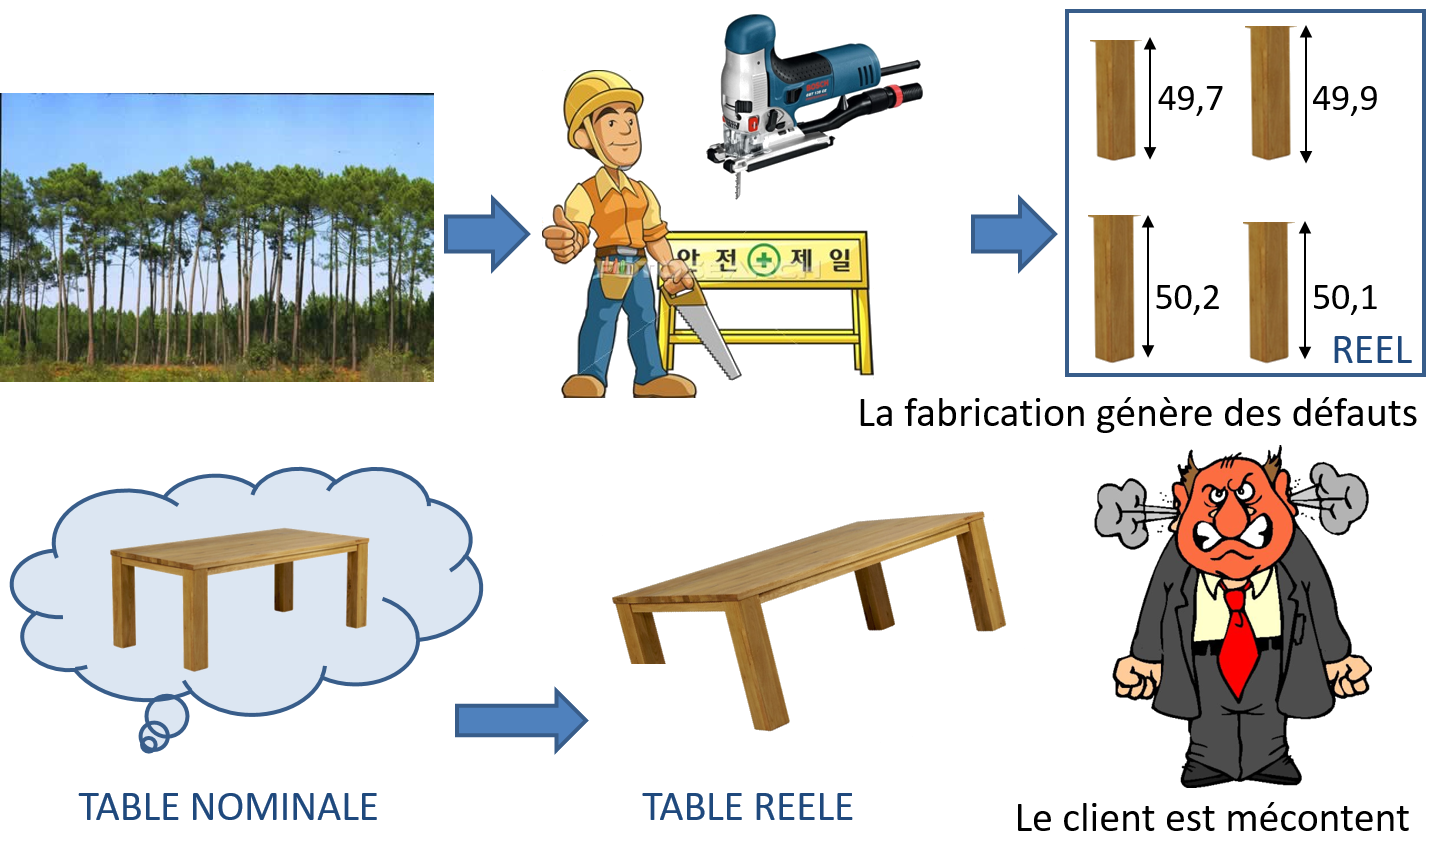
\includegraphics[width=0.9\linewidth]{img/Picture3}
\end{center}
}}

{\frame{
\frametitle{Fabrication}

Première solution: Amélioration des moyens de production.

\begin{center}
 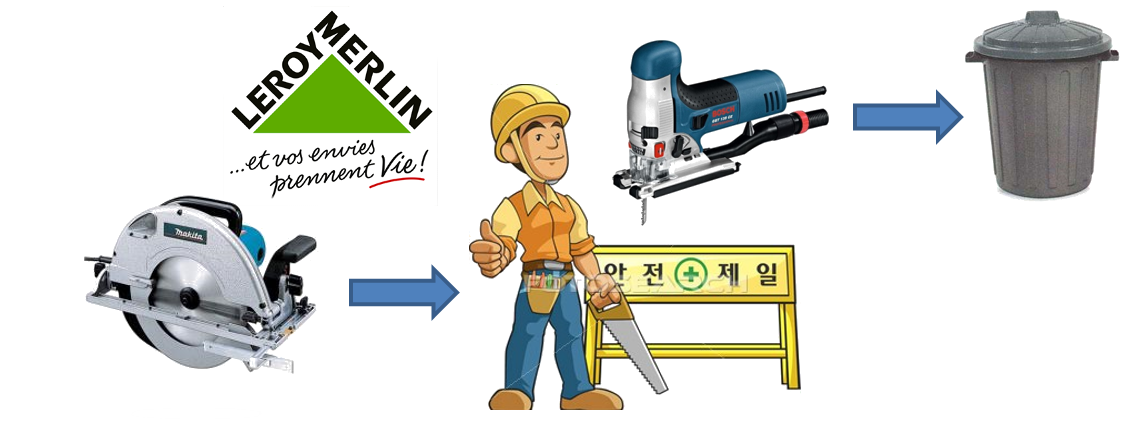
\includegraphics[width=0.9\linewidth]{img/Picture4}
\end{center}

\begin{minipage}{0.45\linewidth}
 \centering 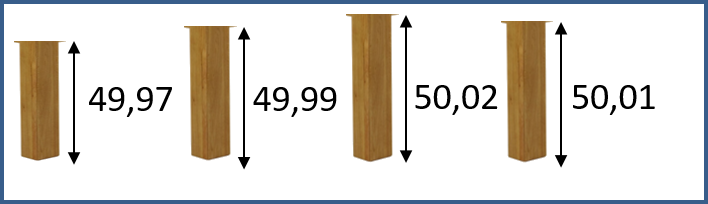
\includegraphics[width=0.9\linewidth]{img/Picture5}
\end{minipage}\hfill
\begin{minipage}{0.45\linewidth}
La table a toujours des défauts, cependant: \\
Répond-t-elle au besoin?
\end{minipage}
}}

{\frame{
\frametitle{Mise en place de niveaux sur les valeurs}

\begin{itemize}
 \item Il est nécessaire de mettre en place des niveaux sur les valeurs des critères,
 \item Ces niveaux sont issus de l'expérience du concepteur, de simulations, d'essais sur des prototypes, etc...
 \item Lorsque les critères sont liés à des valeurs géométriques, il sont appelés spécifications géométriques,
 \item Les niveaux associées sont appelés tolérances géométriques.
\end{itemize}

\begin{minipage}{0.45\linewidth}
 \centering 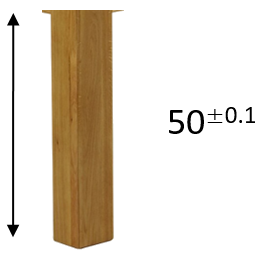
\includegraphics[width=0.5\linewidth]{img/Picture6}
\end{minipage}\hfill
\begin{minipage}{0.45\linewidth}
Spécification: Longueur comprise entre 49,9 et 50,1 mm
\begin{itemize}
 \item Un pied de 49,94 convient,
 \item Un pied de 50,11 ne convient pas.
\end{itemize}
\end{minipage}
}}

{\frame{
\frametitle{Nécessité de normes}

\textbf{Problème:} Comment vérifier que la spécification est vérifiée ?

~\

\begin{minipage}{0.45\linewidth}
 \centering 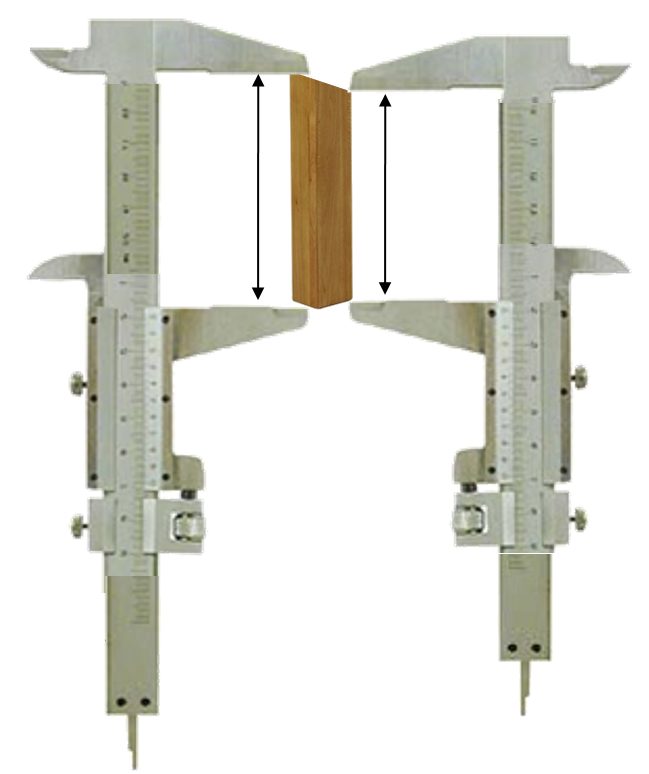
\includegraphics[width=0.9\linewidth]{img/Picture7}
\end{minipage}\hfill
\begin{minipage}{0.45\linewidth}
\begin{itemize}
 \item Les deux mesures ne donnent pas le même résultat,
 \item Le client et le fabriquant ne sont pas d'accord,
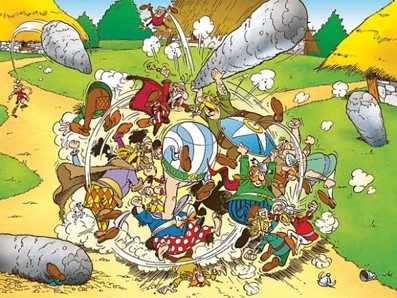
\includegraphics[width=0.5\linewidth]{img/Picture8}
 \item Il faut donc établir des normes pour spécifier les pièces,
 \item Ces spécifications doivent préciser le lien entre la géométrie et le contrôle.
\end{itemize}
\end{minipage}
}}

\section{Spécification tridimensionnelle}

{\frame{
\frametitle{Spécification}

\begin{defi}
Une \textbf{spécification} est une \textbf{condition} sur une \textbf{dimension} définie par une \textbf{caractéristique} sur des \textbf{éléments géométriques} identifiés par des \textbf{opérations} à partir du \textbf{modèle du réel}.
\end{defi}

\begin{itemize}
 \item \textbf{Condition}: Validée ou pas,
 \item \textbf{Dimension:} Valeur d'une caractéristique,
 \item \textbf{Caractéristique:} Angle ou distance,
 \item \textbf{Eléments géométriques:} Point, droite ou plan,
 \item \textbf{Opérations:} Présentées dans la suite,
 \item \textbf{Modèle du réel:} Modèle du réel représenté avec plus ou moins de détail et de réalisme.
\end{itemize}
}}

{\frame{
\frametitle{Eléments géométriques}

\begin{itemize}
 \item La spécification porte sur des éléments géométriques issus du réel,
 \item Le réel de la pièce intègre un certain nombre de défauts:
  \begin{itemize}
 	\item État de surface (rugosité),
 	\item Forme,
 	\item Position,
 	\item Orientation,
  \end{itemize}
 \item Le modèle de la pièce intégrant tous ces défauts est le plus proche du réel,
 \item Le modèle qui n'intègre aucun défaut est le nominal.
\end{itemize}

 \centering 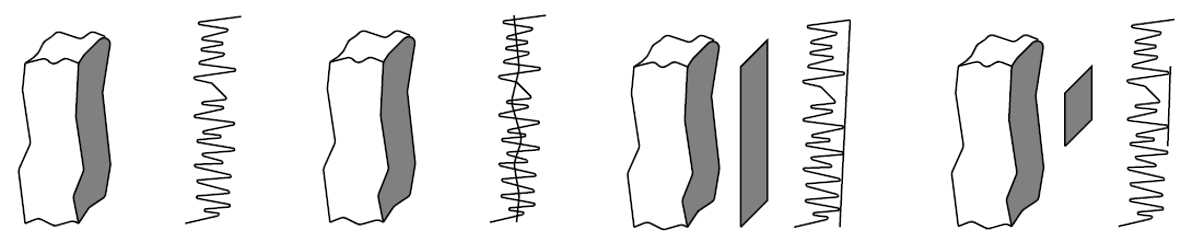
\includegraphics[width=0.9\linewidth]{img/Picture9}
}}

{\frame{
\frametitle{Opérations sur les éléments géométriques}

\begin{itemize}
 \item \textbf{Extraction et la partition:} Parfois, seules certaines parties de ce modèle sont utiles à l'étude, dans ces cas, des opérations d'extraction et de partition sont utiles,
  \item \textbf{Partition:} Consiste à décomposer la pièce en entités
(Ex: Ne considérer qu'une surface d'un volume),
 \item \textbf{Extraction:} Extraire un certain nombre d'entités de la surface
(Ex: Discrétisation d'une pièce (surface) en un nuage de points),
\item Les éléments extraits et partitionnés sont des éléments \textbf{réels},
 \item \textbf{L'association:} Consiste à associer un élément idéal à un élément réel. L'association nécessite la mise en place de contraintes et de critères d'association.
\end{itemize}
}}

{\frame{
\frametitle{Spécification et le tolérancement}

\begin{itemize}
 \item La spécification consiste à proposer de manière univoque des caractéristiques sur une géométrie,
 \item A partir d'un modèle défini d'une pièce, il est possible de mettre en place plusieurs types de spécification selon le besoin:
 \begin{itemize}
 \item Spécifications dimensionnelles,
 \item Spécifications géométriques,
 \end{itemize}
 \item A ces spécifications sont associées des tolérances, intervalles dans lesquelles les valeurs (angles, distances) associées aux spécifications doivent être comprises.
\end{itemize}
}}

{\frame{
\frametitle{Principe de l'indépendance}

\begin{itemize}
 \item Chaque exigence (spécification) dimensionnelle ou géométrique spécifiée sur un dessin doit être respectée en elle-même (indépendamment) sauf si une relation particulière est spécifiée,
  \item Ainsi, sans relation spécifiée, la tolérance géométrique s'applique sans tenir compte de la dimension de l'élément. Les deux exigences sont traitées comme indépendantes.
\end{itemize}
}}

{\frame{
\frametitle{Spécifications dimensionnelles}

\begin{itemize}
 \item \textbf{Définition:} Limite uniquement les dimensions locales réelles d'un élément mais pas ses écarts de forme (mesure entre deux points). Cela ne s'applique qu'a des éléments de type
\begin{itemize}
 \item Cylindre,
 \item Plans parallèles en vis à vis.
\end{itemize}
  \item \textbf{Enveloppe}: Il est possible d'ajouter une exigence d'enveloppe dans le cadre de spécifications dimensionnelles linéaires. Cela implique que l'enveloppe de forme parfaite à la dimension au maximum de matière de l'élément ne soit pas dépassée.
\end{itemize}
}}

{\frame{
\frametitle{Spécifications géométriques}

\begin{itemize}
 \item Les spécifications géométriques consistent à définir une zone de tolérance qui doit contenir tous les points de l'élément réel afin qu'il soit conforme à la spécification,
 \item Une \textbf{zone de tolérance} est une portion de l'espace de géométrie parfaite, devant contenir l'élément réel.
\end{itemize}
}}

{\frame{
\frametitle{Spécifications de forme}

\begin{itemize}
\begin{minipage}{0.45\linewidth}
 \item Une spécification de forme est une zone de tolérance indépendante du reste de la géométrie de la pièce
\end{minipage}\hfill
\begin{minipage}{0.45\linewidth}
 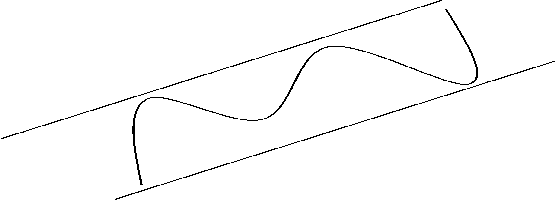
\includegraphics[align=c,width=0.8\linewidth]{img/Picture10},
\end{minipage}
 \item Exemple issu du dessin de définition.
\end{itemize}

\begin{center}
 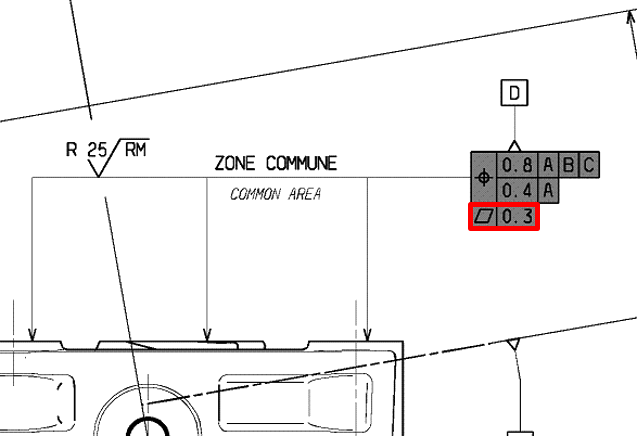
\includegraphics[width=0.6\linewidth]{img/Picture11}
\end{center}
}}

{\frame{
\frametitle{Définir l'orientation/position de la zone}

\begin{itemize}
 \item Parfois, il est nécessaire de définir la position d'une géométrie par rapport à une autre,
 \item Problème: Il est impossible de s'appuyer directement sur une géométrie réelle avec défauts,
 \item Il faut donc définir une géométrie idéale capable de définir l'orientation et/ou la position de la zone de tolérance.
\end{itemize}

\textbf{Mise en place d'une référence}

\begin{itemize}
 \item Une référence est une surface partitionnée et/ou extraite de la pièce (élément réel),
 \item A cette surface un élément idéal est associé,
 \begin{enumerate}
	\item Avec une contrainte par rapport à un autre élément,
	\item Avec une contrainte par rapport à la surface réelle,
	\item Avec un critère d'optimisation.
\end{enumerate}
\end{itemize}


\begin{center}
 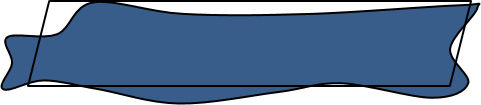
\includegraphics[width=0.4\linewidth]{img/Picture12}
\end{center}
}}

{\frame{
\frametitle{Types de références}

Il existe plusieurs types de références:
\begin{itemize}
 \item Les références simples 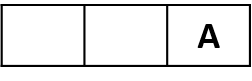
\includegraphics[align=c,width=0.19\linewidth]{img/Picture13},
 \item Les références communes 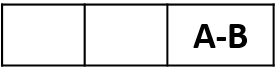
\includegraphics[align=c,width=0.19\linewidth]{img/Picture14}
	\begin{itemize}
 	\item Elément simple formé à partir de plusieurs références
	\end{itemize}
 \item Les systèmes de références spécifiées  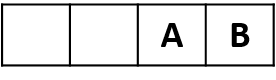
\includegraphics[align=c,width=0.2\linewidth]{img/Picture15},
	\begin{itemize}
	 \item B, référence secondaire, est en position théorique exacte par rapport à A, référence primaire,
	\end{itemize}
 \item Les références partielles 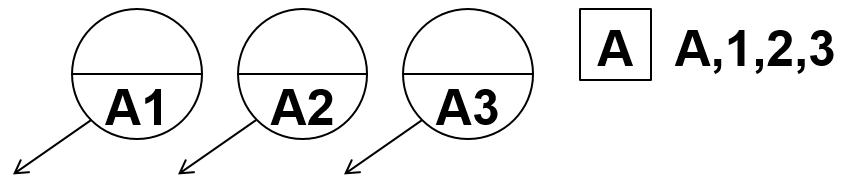
\includegraphics[align=c,width=0.5\linewidth]{img/Picture16}.
\end{itemize}
}}

{\frame{
\frametitle{Systèmes de références}

\begin{center}
 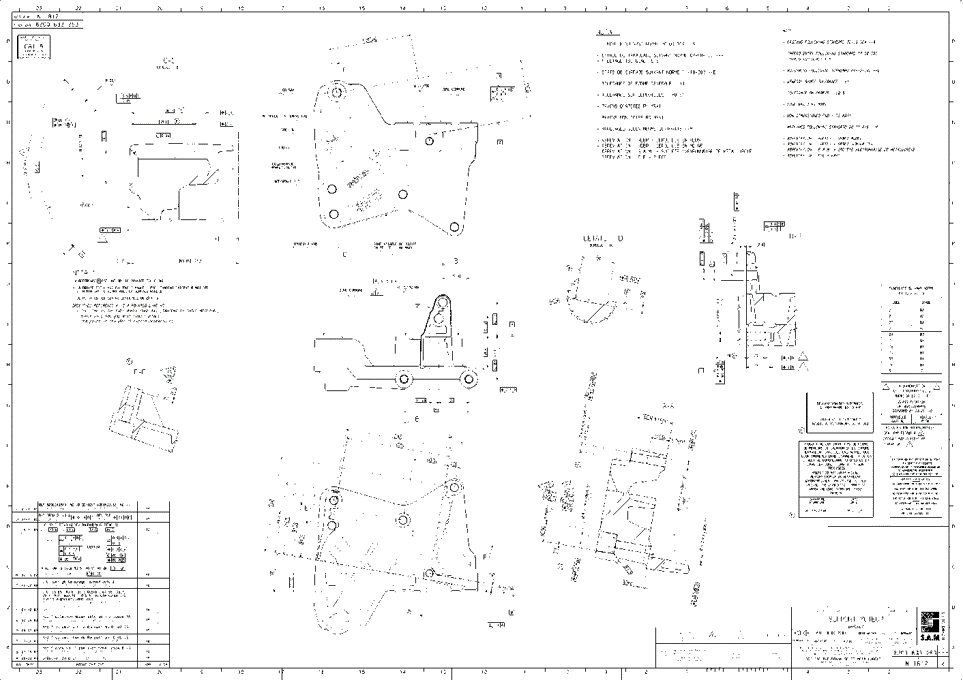
\includegraphics[width=0.7\linewidth]{img/Picture17}
\end{center}

\begin{enumerate}
 \item Trouver les références,
 \item Construire les systèmes de référence,
 \item Déterminer les degrés de mobilité de la pièce au fur et à mesure.
\end{enumerate}
}}

{\frame{
\frametitle{Spécification d'orientation}

\begin{itemize}
 \item Pour ce type de spécifications, seul l'orientation de la référence spécifiée et la zone de tolérance est définie,
 \item Exemple issu du dessin de définition.
\end{itemize}

\begin{center}
 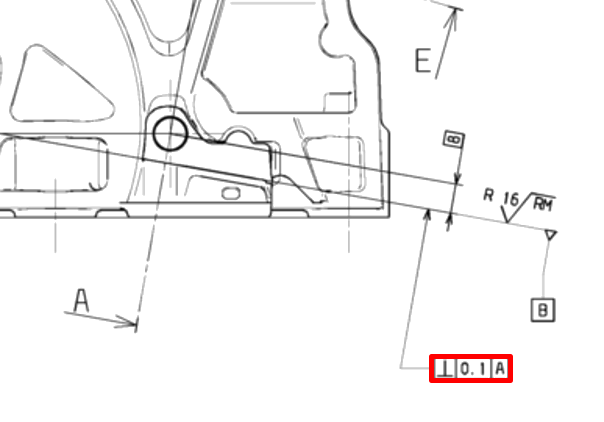
\includegraphics[width=0.7\linewidth]{img/Picture18}
\end{center}
}}

{\frame{
\frametitle{Spécification de position}

\begin{itemize}
 \item Pour ce type de spécifications, la distance entre la référence spécifiée et la zone de tolérance est définie,
 \item Exemple issu du dessin de définition.
\end{itemize}

\begin{center}
 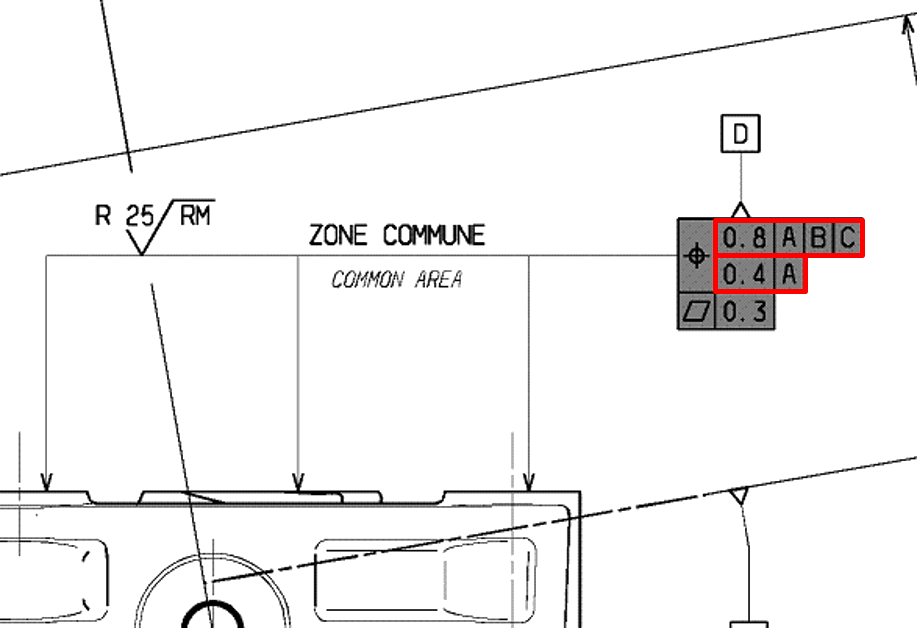
\includegraphics[width=0.7\linewidth]{img/Picture19}
\end{center}
}}

{\frame{
\frametitle{Maximum de matière}

\begin{itemize}
 \item Exception au principe de l'indépendance,
 \item Cette condition implique que l'état virtuel ne soit pas dépassé
 \item Exemple issu du dessin de définition.
\end{itemize}

\begin{center}
 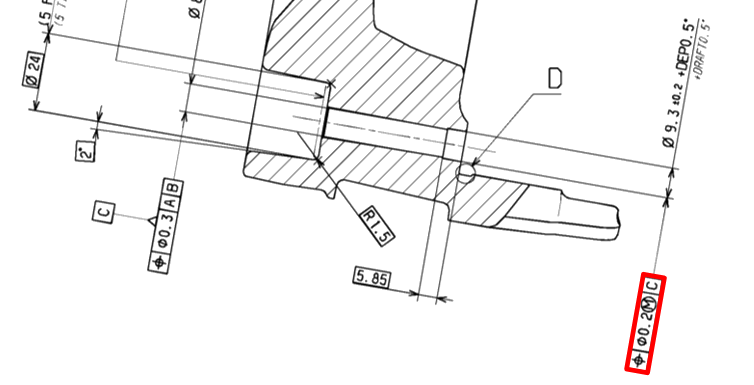
\includegraphics[width=0.7\linewidth]{img/Picture20}
\end{center}
}}

{\frame{
\frametitle{Symboles des spécifications}

{\footnotesize
\begin{tabular}{|p{0.1\linewidth}|p{0.1\linewidth}|p{0.1\linewidth}|p{0.1\linewidth}|p{0.1\linewidth}|p{0.12\linewidth}|p{0.1\linewidth}|}
\hline
Forme & 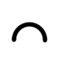
\includegraphics[align=c,width=0.7\linewidth]{img/Picture22} & 
 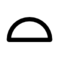
\includegraphics[align=c,width=0.7\linewidth]{img/Picture23} & 
 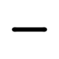
\includegraphics[align=c,width=0.7\linewidth]{img/Picture24} & 
 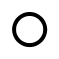
\includegraphics[align=c,width=0.7\linewidth]{img/Picture25} & 
 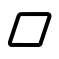
\includegraphics[align=c,width=0.7\linewidth]{img/Picture26} & 
 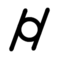
\includegraphics[align=c,width=0.7\linewidth]{img/Picture27} \\
 & Ligne quelconque & Surface quelconque & Rectitude & Circularité & Planéité & Cylindricité \\
\hline
Orientation & 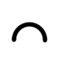
\includegraphics[align=c,width=0.7\linewidth]{img/Picture22} & 
 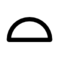
\includegraphics[align=c,width=0.7\linewidth]{img/Picture23} & 
 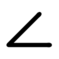
\includegraphics[align=c,width=0.7\linewidth]{img/Picture29} & 
 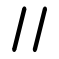
\includegraphics[align=c,width=0.7\linewidth]{img/Picture30} & 
 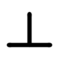
\includegraphics[align=c,width=0.7\linewidth]{img/Picture31} \\
 & Ligne quelconque & Surface quelconque & Inclinaison & Parallélisme & Perpendicularité \\
\cline{1-6}
Position & 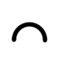
\includegraphics[align=c,width=0.7\linewidth]{img/Picture22} & 
 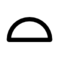
\includegraphics[align=c,width=0.7\linewidth]{img/Picture23} & 
 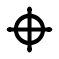
\includegraphics[align=c,width=0.7\linewidth]{img/Picture32} & 
 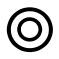
\includegraphics[align=c,width=0.7\linewidth]{img/Picture33} & 
 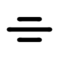
\includegraphics[align=c,width=0.7\linewidth]{img/Picture34} \\
 & Ligne quelconque & Surface quelconque & Localisation & Coaxialité & Symétrie \\
\cline{1-6}
Débattement & 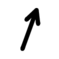
\includegraphics[align=c,width=0.7\linewidth]{img/Picture35} & 
 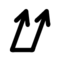
\includegraphics[align=c,width=0.7\linewidth]{img/Picture36} \\
  & Simple & Total \\ 
\cline{1-3}
\end{tabular}}
}}

\section{Spécification une dimension}

{\frame{
\frametitle{Cotation une dimension}

\begin{itemize}
 \item Une dimension $d_{i,j}^k$ c'est :
 \begin{itemize}
  \item une grandeur mesurée représentée par une valeur (élément de R) note $g_{i,j}$,
  \item une position géométrique notée par les indices $i,j$ correspondant aux indices $i$ et $j$ des deux points considérés,
  \item une pièce ou un assemblage désigné par l'exposant $k$.
 \end{itemize}
 \item Une cote réelle $C_{i,j}^*$ est une suite ordonnée d'un nombre fini de dimensions. $i,j$ est l'indice définissant la position géométrique de la cote réelle.
 \begin{itemize}
  \item $C_{1,2}:(d_{1,2}^1,d_{1,2}^2,d_{1,2}^3,...,d_{1,2}^p)$,
  \item $C_{1,3}:(d_{1,3}^1,d_{1,3}^2,d_{1,3}^3,...,d_{1,3}^p)$.
 \end{itemize}
\end{itemize}

\begin{center}
 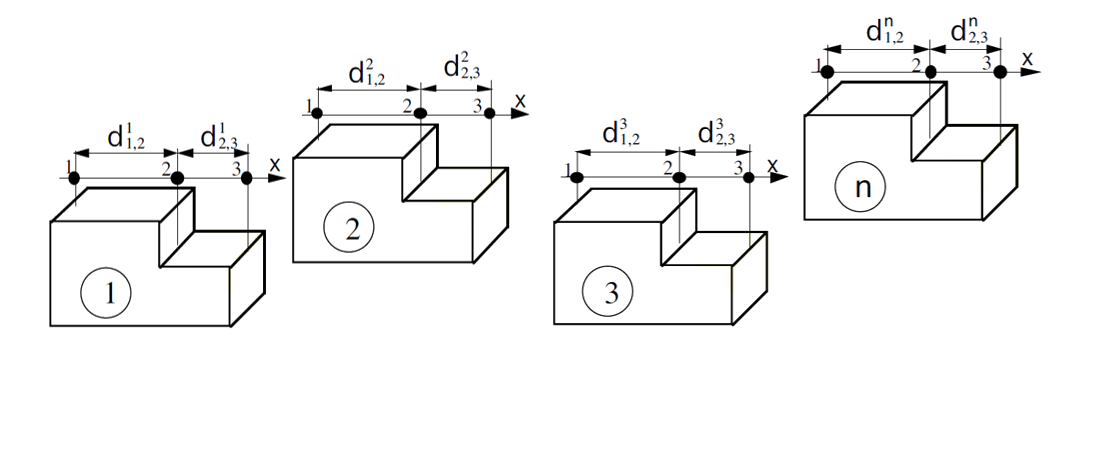
\includegraphics[width=0.8\linewidth]{img/Picture37}
\end{center}
}}

{\frame{
\frametitle{Opérations sur les cotes unidirectionnelles}

\begin{itemize}
 \item Somme: Avec une chaine fermée de 3 cotes $C_{1,2}^*$, $C_{2,3}^*$, $C_{3,1}^*$. Sur la k\textsuperscript{ème} pièce, la valeur $g_{i,j}$ de l'une des trois dimensions $d_{1,2}^k$, $d_{2,3}^k$, et $d_{3,1}^k$ peut-être déduite des valeurs des deux autres dimensions.\\
\begin{minipage}{0.45\linewidth}
 \begin{itemize}
  \item $g_{1,3} = g_{1,2} + g_{2,3}$,
  \item $g_{1,2} = g_{1,3} - g_{2,3}$,
  \item $g_{2,3} = g_{1,3} - g_{1,2}$.
 \end{itemize}
\end{minipage}\hfill
\begin{minipage}{0.45\linewidth}
 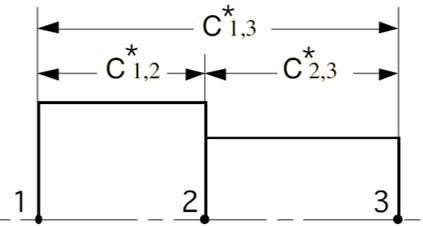
\includegraphics[width=0.8\linewidth]{img/Picture38}
\end{minipage}
 \item Inclusion: La dimension $d_{i,j}^k$ sera incluse dans la cote réelle
	\begin{itemize}
	 \item $C_{i,j}^*$ : ($d_{i,j}^1$,$d_{i,j}^2$,$d_{i,j}^3$,...,$d_{i,j}^p$) si $d_{i,j}^k$ a sa valeur $g_{i,j}^k$ comprise entre la plus grande et la plus petite des valeurs prises par les dimensions de la cote,
	 \item $C_{i,j}^*$ : ${g_{i,j}^l}_{mini} \leq g_{i,j}^k \leq {g_{i,j}^m}_{maxi}$,
	 \item $C_{i,j}^{*'} \subset C_{i,j}^{*}$,
	 \item Une cote $C_{i,j}^{*'}$ sera incluse dans une cote $C_{i,j}^{*}$ si toutes les dimensions de la cote $C_{i,j}^{*'}$ sont incluses dans la cote $C_{i,j}^{*}$.
	\end{itemize}
\end{itemize}
}}

{\frame{
\frametitle{Opérations sur les cotes unidirectionnelles}

\begin{itemize}
 \item Afin de systématiser la mise en équation des chaines de cotes il est possible d'utiliser la représentation vectorielle suivante :
 \begin{itemize}
  \item la cote condition désigne la cote dépendante (flèche a double trait),
  \item les cotes indépendantes sont des vecteurs (flèches à simple trait),
  \item la cote condition est le vecteur résultant de la somme vectorielle des cotes indépendantes de la chaine.
 \end{itemize}
\begin{minipage}{0.6\linewidth}
 \begin{itemize}
 \item Relation vectorielle sur x
 \begin{itemize}
  \item $f_{2,3} = a_{2,8} - b_{8,6} - c_{6,4} - d_{4,3}$,
 \end{itemize}
 \item Relations entre les valeurs des cotes maxi et mini :
 \begin{itemize}
  \item ${f_{2,3}}_{maxi} = {A_{2,8}}_{maxi} - {B_{8,6}}_{mini} - {C_{6,4}}_{mini} - {D_{4,3}}_{mini}$,
  \item ${f_{2,3}}_{mini} = {A_{2,8}}_{mini} - {B_{8,6}}_{maxi} - {C_{6,4}}_{maxi} - {D_{4,3}}_{maxi}$,
 \end{itemize} 
 \item Relation entre les intervalles de tolerances :
 \begin{itemize}
  \item $IT(f_{2,3}) = IT(A_{2,8}) + IT(B_{8,6}) + IT(C_{6,4}) + IT(D_{4,3})$
 \end{itemize}
\end{itemize}
\end{minipage}\hfill
\begin{minipage}{0.35\linewidth}
 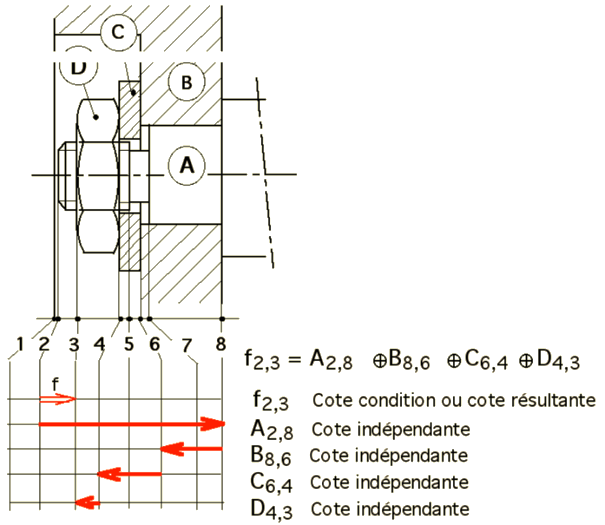
\includegraphics[width=\linewidth]{img/Picture39}
\end{minipage}
\end{itemize}
}}

\section{Méthode de spécification}

{\frame{
\frametitle{Méthode de spécification}

Les étapes suivantes permettent de générer une spécification:
\begin{enumerate}
 \item Définition du mécanisme (géométrie),
 \item Définition de la mise en position des pièces,
 \item Mise en place des exigences,
 \item Pour chaque exigence, une chaine de cote 3D,
 \item Mise en place des spécifications.
\end{enumerate}
}}

{\frame{
\frametitle{Définition de la mise en position}

\begin{itemize}
 \item Comment les pièces sont positionnées?
 \item Le concepteur doit définir la mise en position des pièces du mécanisme
 \item Il peut pour cela s'aider d'informations:
 \begin{itemize}
  \item l'assemblage du mécanisme,
  \item les exigences,
  \item ...
 \end{itemize}
 \begin{minipage}{0.45\linewidth}
  \item Ex: Qu'est ce qui définie la position de l'arbre dans le mécanisme suivant?
 \end{minipage}\hfill
 \begin{minipage}{0.45\linewidth}
  \centering  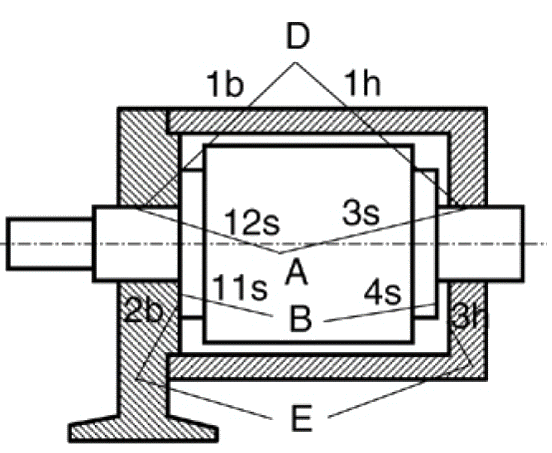
\includegraphics[width=\linewidth]{img/Picture40} 
 \end{minipage}
\end{itemize}
}}

{\frame{
\frametitle{Mise en place des spécifications}

\begin{itemize}
 \item En fonction de la mise en position, les premières spécification liées à l'assemblage peuvent être mises en place,
  \begin{itemize}
  \item cf Tableau (Bernard Anselmetti)
 \end{itemize}
 \item Le reste des spécifications sont déterminées à partir des exigences.
\end{itemize}
}}

{\frame{
\frametitle{Tableau des spécifications}

\begin{center}
 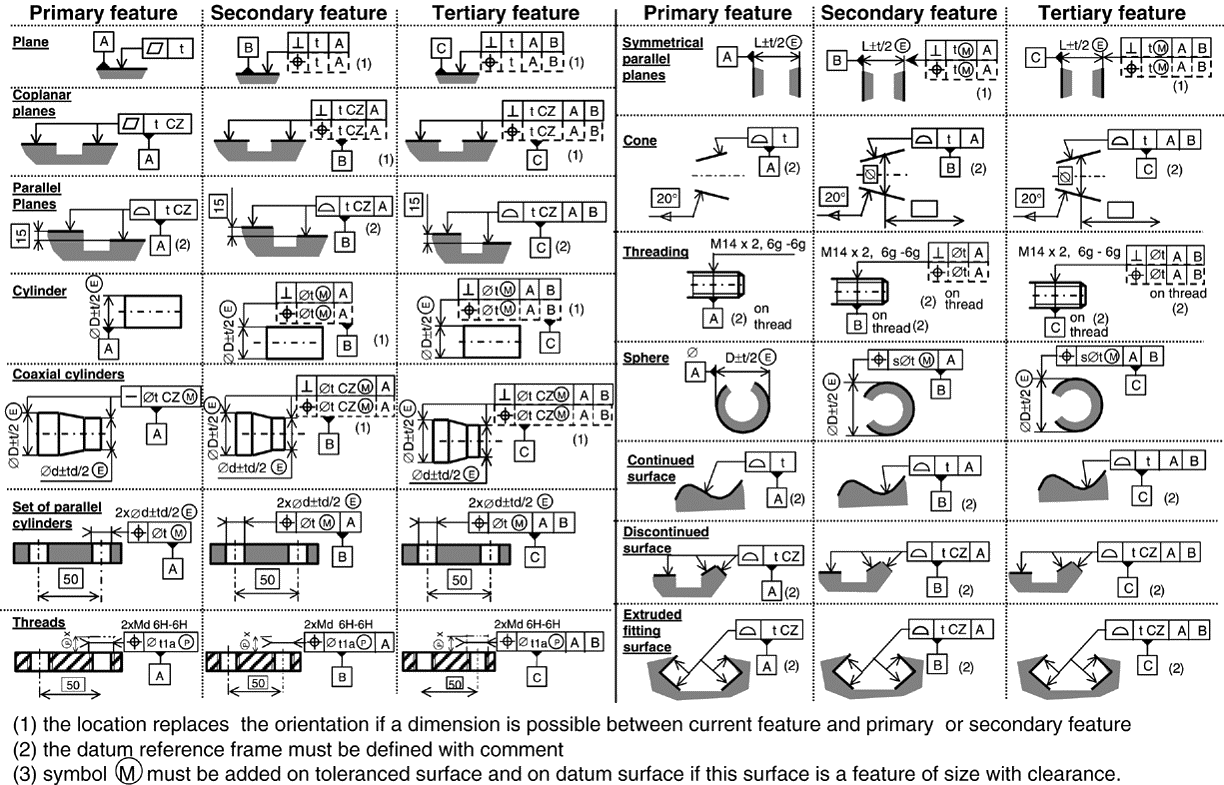
\includegraphics[width=\linewidth]{img/Picture41}
\end{center}
}}

{\frame{
\frametitle{Les spécifications géométriques}

\begin{savoir}
Vous devez être capables :
\begin{itemize}
 \item de déterminer les défauts potentiels d'une pièce,
 \item de modéliser l'impact de ces défauts à l'aide de torseurs de petits déplacements.
\end{itemize}
\end{savoir}

\begin{prob}

Il est nécessaire d'utiliser d'autres formes de représentation d'un mécanisme.
\begin{itemize}
 \item \textit{Problème: Comment limiter les défauts géométriques ?}
 \item \textbf{Perspectives}: Déterminer les spécifications géométriques sur une pièce.
\end{itemize}
\end{prob}

}}


\end{document}